% figures/new/fig_schedules.tex -- Figure 3 (fig:schedules), written by W3. Self-contained float (BLUEPRINT 2.7, Override O6).
% Built only from printed cells of tables/DRC_visualization_4.tex (benefit as a percentage of the PIA at claiming ages 62-70):
%   AN0 (NRA at 65), line 37:      80, 86.67, 93.33, 100, 104.5, 109, 113.5, 118, 122.5
%   AN2 (NRA at 67), line 39:      70, 75, 80, 86.67, 93.33, 100, 104.5, 109, 113.5
%   AD5 (DRC at 10%), line 47:     80, 86.67, 93.33, 100, 110, 120, 130, 140, 150
%   AL4 (Linear +/-10%), line 53:  70, 80, 90, 100, 110, 120, 130, 140, 150
% House style: width 9cm, grid, legend below the axis; colors are the FROT palette defined in preamble.tex.
\begin{figure}[!t]
\centering
\caption{Benefit Schedules under the Status Quo, a Higher NRA (AN2), a Higher DRC (AD5), and a Symmetric $\pm 10$ Percent Adjustment (AL4)}
\label{fig:schedules}
\vspace{6pt}
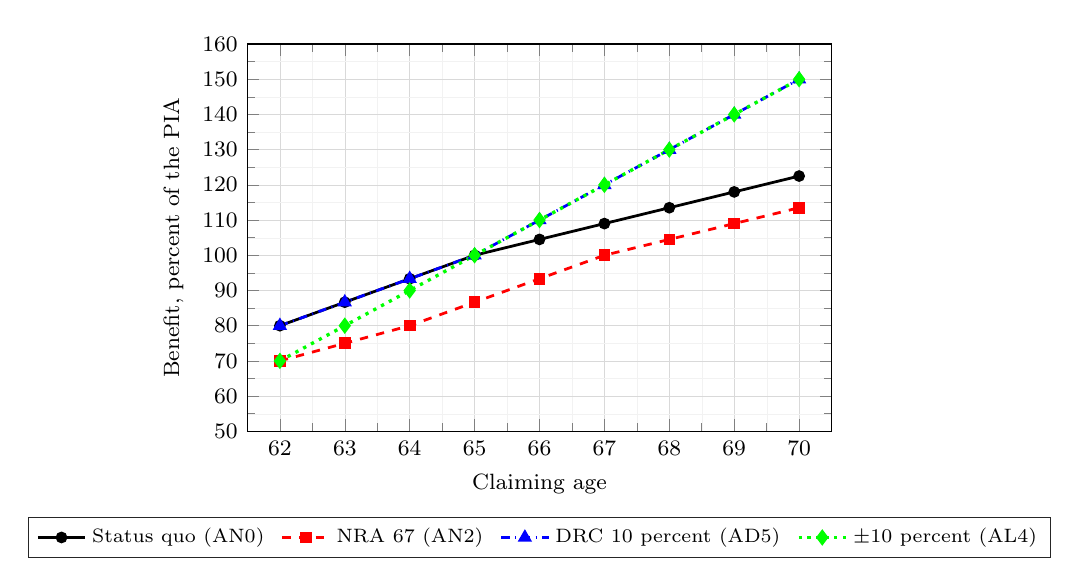
\begin{tikzpicture}
\begin{axis}[%
width=9cm,
height=6.5cm,
xlabel={Claiming age},
ylabel={Benefit, percent of the PIA},
xmin=61.5, xmax=70.5,
ymin=50, ymax=160,
xtick={62,63,...,70},
ytick={50,60,...,160},
grid=both,
grid style={line width=0.2pt, draw=gray!30},
minor grid style={line width=0.1pt, draw=gray!10},
minor tick num=1,
axis background/.style={fill=white},
legend style={at={(0.5,-0.22)}, anchor=north, legend columns=4, draw=white!15!black, font=\scriptsize, /tikz/every even column/.append style={column sep=0.4em}},
legend cell align=left,
tick label style={font=\footnotesize},
label style={font=\footnotesize}
]
% AN0, status quo (NRA 65, DRC 4.5 percent)        % src: tables/DRC_visualization_4.tex:37
\addplot [color=black, line width=1pt, mark=*, mark size=1.6pt] coordinates {(62,80) (63,86.67) (64,93.33) (65,100) (66,104.5) (67,109) (68,113.5) (69,118) (70,122.5)};
\addlegendentry{Status quo (AN0)}
% AN2, NRA at 67                                  % src: tables/DRC_visualization_4.tex:39
\addplot [color=red, dashed, line width=1pt, mark=square*, mark size=1.6pt, mark options={solid}] coordinates {(62,70) (63,75) (64,80) (65,86.67) (66,93.33) (67,100) (68,104.5) (69,109) (70,113.5)};
\addlegendentry{NRA 67 (AN2)}
% AD5, DRC at 10 percent                          % src: tables/DRC_visualization_4.tex:47
\addplot [color=blue, dash dot, line width=1pt, mark=triangle*, mark size=2pt, mark options={solid}] coordinates {(62,80) (63,86.67) (64,93.33) (65,100) (66,110) (67,120) (68,130) (69,140) (70,150)};
\addlegendentry{DRC 10 percent (AD5)}
% AL4, symmetric +/-10 percent                     % src: tables/DRC_visualization_4.tex:53
\addplot [color=green, dotted, line width=1.2pt, mark=diamond*, mark size=2pt, mark options={solid}] coordinates {(62,70) (63,80) (64,90) (65,100) (66,110) (67,120) (68,130) (69,140) (70,150)};
\addlegendentry{$\pm 10$ percent (AL4)}
\end{axis}
\end{tikzpicture}
\begin{minipage}{0.92\textwidth}
\vspace{4pt}
\scriptsize
\textit{Notes:} Social Security retirement benefit payable at each claiming age, as a percentage of the primary insurance amount (PIA), from \autoref{tab:schedules}. The status quo is the schedule of the 1920--1940 cohorts, with a normal retirement age (NRA) of 65, a reduction of 6.67 percentage points per year of claiming before the NRA, and a delayed retirement credit (DRC) of 4.5 percentage points per year after it. AN2 raises the NRA to 67; AD5 raises the DRC to 10 percent per year and leaves the schedule through age 65 unchanged; AL4 sets the reduction and the credit equal to 10 percent per year, so the schedule coincides with AD5 after the NRA and lies below the status quo before it. AD5 and AL4 coincide at ages 65--70. Sources: rules of the Social Security Administration (status quo) and the reform definitions of \autoref{tab:menu}.
% src: tables/DRC_visualization_4.tex:37,39,47,53; 7_policy_reforms.tex:90 (6.67 and 4.5 pp)
\end{minipage}
\end{figure}
